\documentclass[uplatex, 12pt, a4paper, dvipdfmx]{jsarticle}
\title{圏と層 斎藤毅\\講義ノート}
\author{司馬博文 J4-190549\\hirofumi-shiba48@g.ecc.u-tokyo.ac.jp}
\date{\today}
\pagestyle{headings}
\usepackage[top=15truemm,bottom=15truemm,left=10truemm,right=10truemm]{geometry}
\usepackage{amsmath, amsfonts, amsthm, mathptmx, amssymb, ascmac, amscd, color, comment, tikz-cd}
\newtheorem{theorem}{定理} \newtheorem{definition}{定義} \newtheorem{proposition}{命題} \newtheorem{corollary}[proposition]{系} \newtheorem{lemma}[proposition]{補題} \setcounter{secnumdepth}{4}
% \coprodをmathptmx(文書のフォントをTimesにするpackage)でも使えるようにするために.
\DeclareSymbolFont{cmletters}{OML}{cmm}{m}{it}
\DeclareSymbolFont{cmsymbols}{OMS}{cmsy}{m}{n}
\DeclareSymbolFont{cmlargesymbols}{OMX}{cmex}{m}{n}
\DeclareMathSymbol{\myjmath}{\mathord}{cmletters}{"7C}
\DeclareMathSymbol{\myamalg}{\mathbin}{cmsymbols}{"71}
\DeclareMathSymbol{\mycoprod}{\mathop}{cmlargesymbols}{"60}
\let\jmath\myjmath
\let\amalg\myamalg
\let\coprod\mycoprod

\begin{document}
\maketitle

\part{圏}

\begin{quotation}
    位相空間のホモロジー理論を創始したポアンカレの言葉に「数学とは異なるものを同じとみなす技術である」というものがある.この言葉は色々な解釈ができると思うが,自然科学のいろんな場面で似た形で現れる数学的現象の本質を抽出して抽象化し,一つの理論にまとめることはまさに「異なるものを同じとみなす技術」ではないだろうか.例えば,平面幾何学における相似拡大,解析学における関数のある点の近くでの一次近似,自然科学,経済学の様々な場面で現れる諸量の比例関係などの中に潜む線型性という本質を捉え,抽象化して理論としてまとめたものが線形代数学である.このように抽象化して理論をまとめておくことで数学的現象の本質の理解が深まり,また,新たな現象が見つかった時には,その理論が適用可能であることさえ確かめれば,同じ考察を再び繰り返すことなく抽象化された理論の恩恵を受けることができる.線形代数学が自然科学のあらゆる分野において重要なものであることはいうまでもないであろう.\footnote{志甫淳『層とホモロジー代数』(共立出版,2016)前文}
\end{quotation}
これから,圏論を数学理論として,数学の体系の中で展開して理解を深めていくが,圏とは極めて普遍的な枠組みである.人の世界を認識する要素のうち,極めて基本的なもの,「対象」とそれを結ぶ「射」にまで遡って,そこにある「型」を,圏として捕まえて定式化する.\\

\section{集合とGrothendieck宇宙,写像とfiber積}
圏論の理論をこれから展開していく訳ではあるが,何を基礎として展開するべきであろうか?\\
圏論は,集合論自体も考察の対象として取るわけだから,圏論の考察を展開する際に基盤とする数学的枠組みとしての集合論との関係には注意が必要である.\\
展開法は2つある.集合論の「クラス」の概念を援用して,クラスも含めた取り扱いをすること.こちらは集合論への習熟も必要とするから,今回は執らない.2つ目は「集合」の範囲を,「集合の集合は集合」が成り立つような或る宇宙$mathfrak{U}$の中に限れば,とりあえず基盤としては十分である.しかし,それに当たっては,集合論のZFC公理系にもう1つ公理を付け加えてから,それを集合の定義とせねばならない.\\
以上の議論を定義にまとめる.

\begin{shadebox}\begin{definition}[Grothendieck宇宙]
    空でない集合$\mathfrak{U}$が宇宙であるとは,以下の4条件を充たすことをいう.\\
    1, [推移的集合である]$\forall x,y \; [x\in y \wedge \; y\in \mathfrak{U} \Longrightarrow x\in \mathfrak{U}]$\\
    2, [生成規則:pairing]$\forall x,y \; [x,y\in \mathfrak{U} \Longrightarrow \{ x,y\} \in \mathfrak{U}]$\\
    3, [生成規則:power]$\forall x \; [x\in\mathfrak{U} \Longrightarrow \mathcal{P}(x):=\{ y:\; y \subset x\} \in \mathfrak{U}]$\\
    4, [生成規則:union]$\forall I,x_i \in \mathfrak{U}(i\in I) \; [\; \bigcup_{i\in I} x_i := {y:\; \exists i\in I \; y\in x_i}]$
\end{definition}\end{shadebox}

この4つの公理の下では,以下の命題は全て成り立つ(含意されている).
\begin{shadebox}
    5, $\varnothing\in\mathfrak{U}$
    6, $\forall x\in\mathfrak{U} \; [x\in\mathfrak{U}\Longrightarrow \{ x \} \in \mathfrak{U}]$\\
    7, $\forall x\in\mathfrak{U} \; [x\in\mathfrak{U}\Longrightarrow \bigcup_{y\in x}y\in\mathfrak{U}]$\\
    8, $\forall x,y\in\mathfrak{U} \; [x,y \in\mathfrak{U}\Longrightarrow x\times y\in\mathfrak{U}]$\\
    9, $\forall x,y\in\mathfrak{U} [x\in\mathfrak{U} \wedge y\subset x \Longrightarrow y\in\mathfrak{U}]$\\
    10, $\forall I,x_i\in\mathfrak{U}(i\in I) [I,x_i\in\mathfrak{U}(i\in I)\Longrightarrow \prod_{i\in I}x_i , \coprod_{i\in I}x_i\in\mathfrak{U}]$
\end{shadebox}

\begin{shadebox}\begin{definition}[(小さな)集合]集合とは,ZFC公理系を充たすもののことである.小さな集合とは,ZFC公理系に以下の公理を付け加えた公理系を充たすものである.噛み砕けば,物の集まり$X,Y$と,その元$x\in X$のことである.また,$X=Y$とは,$x\in X \Longleftrightarrow x \in Y$となることの略記である.$$\forall x,y \; [ \forall z (z\in x \Longleftrightarrow z\in y) \Longrightarrow x=y ] \hspace{3mm}\mathrm{(extentionality)}$$
\begin{center}[公理:\rm{Grothendieck宇宙の存在}]$\mathbb{N}\in\mathfrak{U}$を充たす宇宙$\mathfrak{U}$は存在する.\end{center} \vspace{1mm}
\end{definition}\end{shadebox}
こうして存在を保証した宇宙$\mathfrak{U}$を1つ取り,固定する.以降,「小さな集合」と言った場合は,この宇宙$\mathfrak{U}$に所属する集合のことを言う.公理より,$\mathbb{N}$のみならず,そこから構成可能な$\mathbb{Z,Q,R,C}$は全て小さな集合である.一方で,$\mathfrak{U}$自身は勿論,一元集合$\{ \mathfrak{U} \}$も小さくない.
\begin{shadebox}\begin{definition}[写像]写像とは,2つの集合$X,Y$について,$X$の各元$x$に対して$Y$の元$f(x)$が唯一つ定まっている時,$f$を$X$から$Y$への写像と呼び,$f:X\longrightarrow Y$で表す.\end{definition}\end{shadebox}
この$f$に対して,$X$を始域,$Y$を終域と呼ぶ.
なお,2つの写像$f,g:X\longrightarrow Y$が等しいとは,$f=g\Longleftrightarrow \forall x \in X \; [f(x)=g(x)]$と定められる.集合論の言葉で言えば「グラフが等しい」ことを,写像が等しいと定義する.
\begin{shadebox}\begin{definition}[写像の合成]2つの写像$f:X\longrightarrow Y, g:Y\longrightarrow Z$に対し,その合成写像$h:X\longrightarrow Z$が$\forall x \in X \; [h(x)=g(f(x))]$によって定めることができる.以降この$h$を$g\circ f$と書く.\end{definition}\end{shadebox}
\begin{shadebox}\begin{definition}[集合の積]2つの集合$X,Y$に対して,$X\times Y:=\{ (x,y) :\; x\in X \wedge y\in Y\}$と定義する.但し,$(x,y)=(x',y')\Longleftrightarrow x=x'\wedge y=y'$と定義する. \end{definition}\end{shadebox}
集合論的立場からは,$(x,y):=\{\{x\},\{x,y\}\}$と思えば良い.これを順序対,あるいは2-組という.
\begin{shadebox}\begin{definition}[写像の可換図式]$X,Y,W,Z$を集合とし,$f,g,h,k$を写像とする.以降$f:X\longrightarrow Y$を$X\xrightarrow{f}Y$とも書くこととする.この時,以下の図が可換図式であるとは,$h\circ f=k\circ g \Longleftrightarrow \forall x\in X \; [h\circ f(x)=k\circ g(x) \in W]\cdots\star^1$となることと定義する.
    $$ \begin{tikzcd}
        X \arrow[r, "f"] \arrow[d, "g"'] \arrow[dr, phantom, "\circlearrowright"] &  Y \arrow[d, "h"] \\
            Z \arrow[r, "k"] &    W \\
    \end{tikzcd} $$
\end{definition}\end{shadebox}
つまり,図式を有向グラフ(集合$X,Y,W,Z$を頂点,写像$f,g,h,k$を辺とした有向グラフ)だと思った時に,全ての有向道(directed path)が,写像の合成について,"等しい"(定義2の注釈参照)写像を与えるような図式を,可換図式という.「可換」であることの意味は強い,単に始域と終域が等しいだけでは足りない.\\
\textcolor{blue}{*図式の可換性は上のように定義した後,その集合論的な着地点$\star^1$を忘れ去ることが出来るはずだ.無理だろうか.}
\begin{shadebox}\begin{definition}[fiber積]終域が等しい2つの写像$f:X\longrightarrow S, g:Y\longrightarrow S$について,その\rm{fiber積}$X_f\underset{S}{\times_g}Y$を,$$X_f\underset{S}{\times_g}Y:=\{ (x,y)\in X\times Y:\; f(x)=f(y)\in S \}$$  \end{definition}\end{shadebox}
fiberとは(集合論で)単に逆像のことを意味する.2つの写像の,共通する終域$S$の各元$s$についての逆像$f^{-1}(s)=\{ x\in X:\; f(x)=s \},g^{-1}(s)$同士の積$f^{-1}(s)\times g^{-1}(s)$を,全ての$s\in S$について足し合わせたもの(和集合,或いは結びのこと)に他ならない.$$X_f\underset{S}{\times_g}Y=\bigcup_{s\in S}f^{-1}(s)\times g^{-1}(s)$$

\clearpage

\section{圏の定義}
\begin{shadebox}\begin{definition}[圏]圏とは,集合$C,M$と写像$s,t,c,e$の6-組$(C,M,s,t,c,e)$であって,図\ref{def-cd:1} \ref{def-cd:2} \ref{def-cd:3} \ref{def-cd:4}の可換図式を充たすもののことである.但し,$s,t,c,e$は夫々,\begin{eqnarray*}s:M\longrightarrow C,\hspace{5mm} t:M\longrightarrow C, \hspace{5mm} e:C\longrightarrow M\\[3mm] \left. 
\begin{array}{ccc}
    c:M_s\underset{C}{\times_t}M & \stackrel{c}{\longrightarrow} & M \\
    \rotatebox{90}{$\in$} & & \rotatebox{90}{$\in$} \\
    (g,f) & \longmapsto & c(g,f)
\end{array} \right. \hspace{10mm} \end{eqnarray*}を充たす写像である.

\vspace{1mm} \end{definition}\end{shadebox}

\begin{figure}[ht] \begin{center}  \caption{\label{def-cd:1} 射の合成$c$の定義.$s(f)=s(c(g,f))\wedge t(g)=t(c(g,f))$を表す可換図式.}
    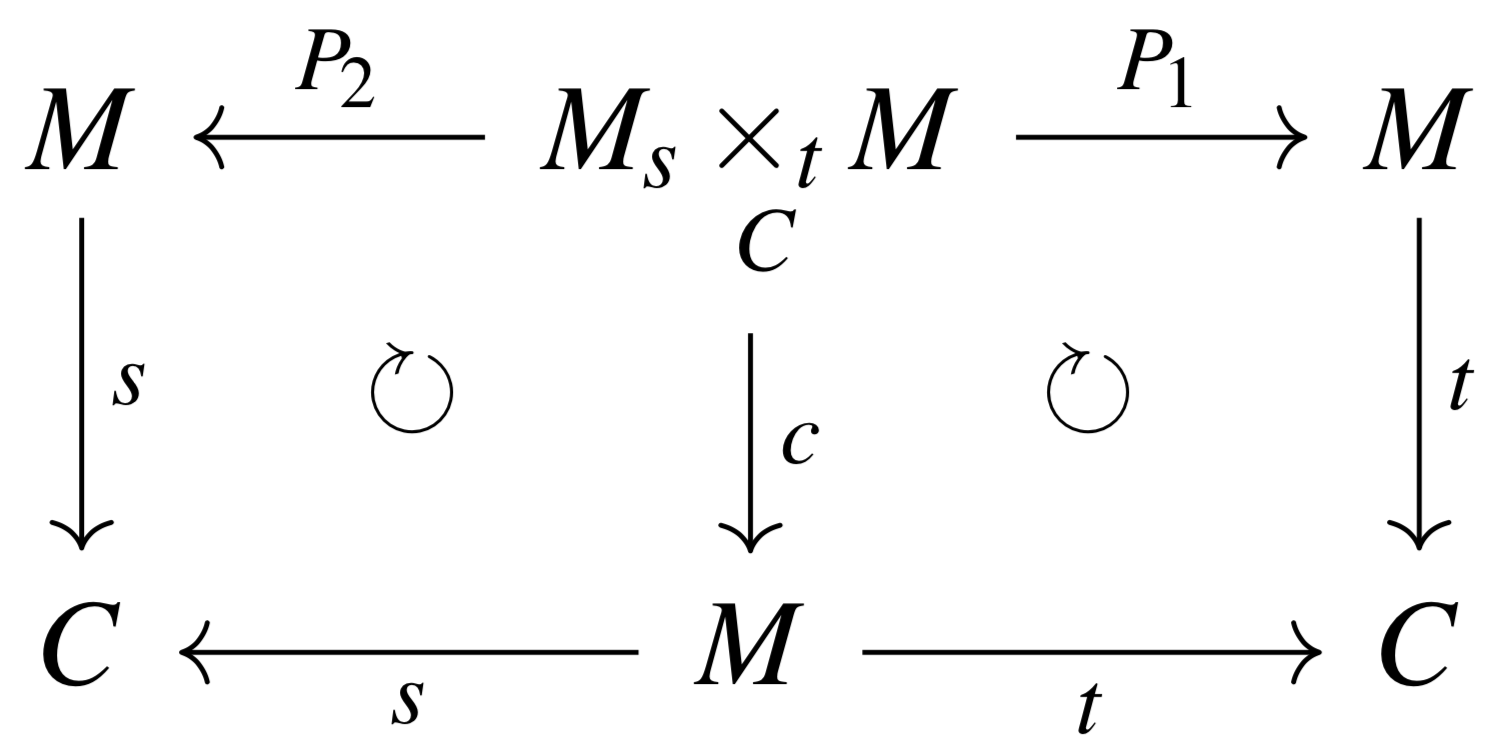
\includegraphics[width=7cm]{cd-1.png}
\end{center}\end{figure}
以降この$P_1, P_2$のことを射影(\underline{p}rojection)と呼ぶ.\hspace{6mm}$P_1: X\underset{S}{\times}Y \longrightarrow X, \; \; \; P_2: X\underset{S}{\times}Y \longrightarrow Y$\\
なお,$M_s\underset{C}{\times_t}M$は2-組で,第1成分が$g$,第2成分が$f$に当たることに注意.

\begin{figure}[ht] \begin{center}  \caption{\label{def-cd:2} 射の合成$c$についての結合則の成立$c(c(h,g),f)=c(h,c(g,f))$を表す可換図式.}
    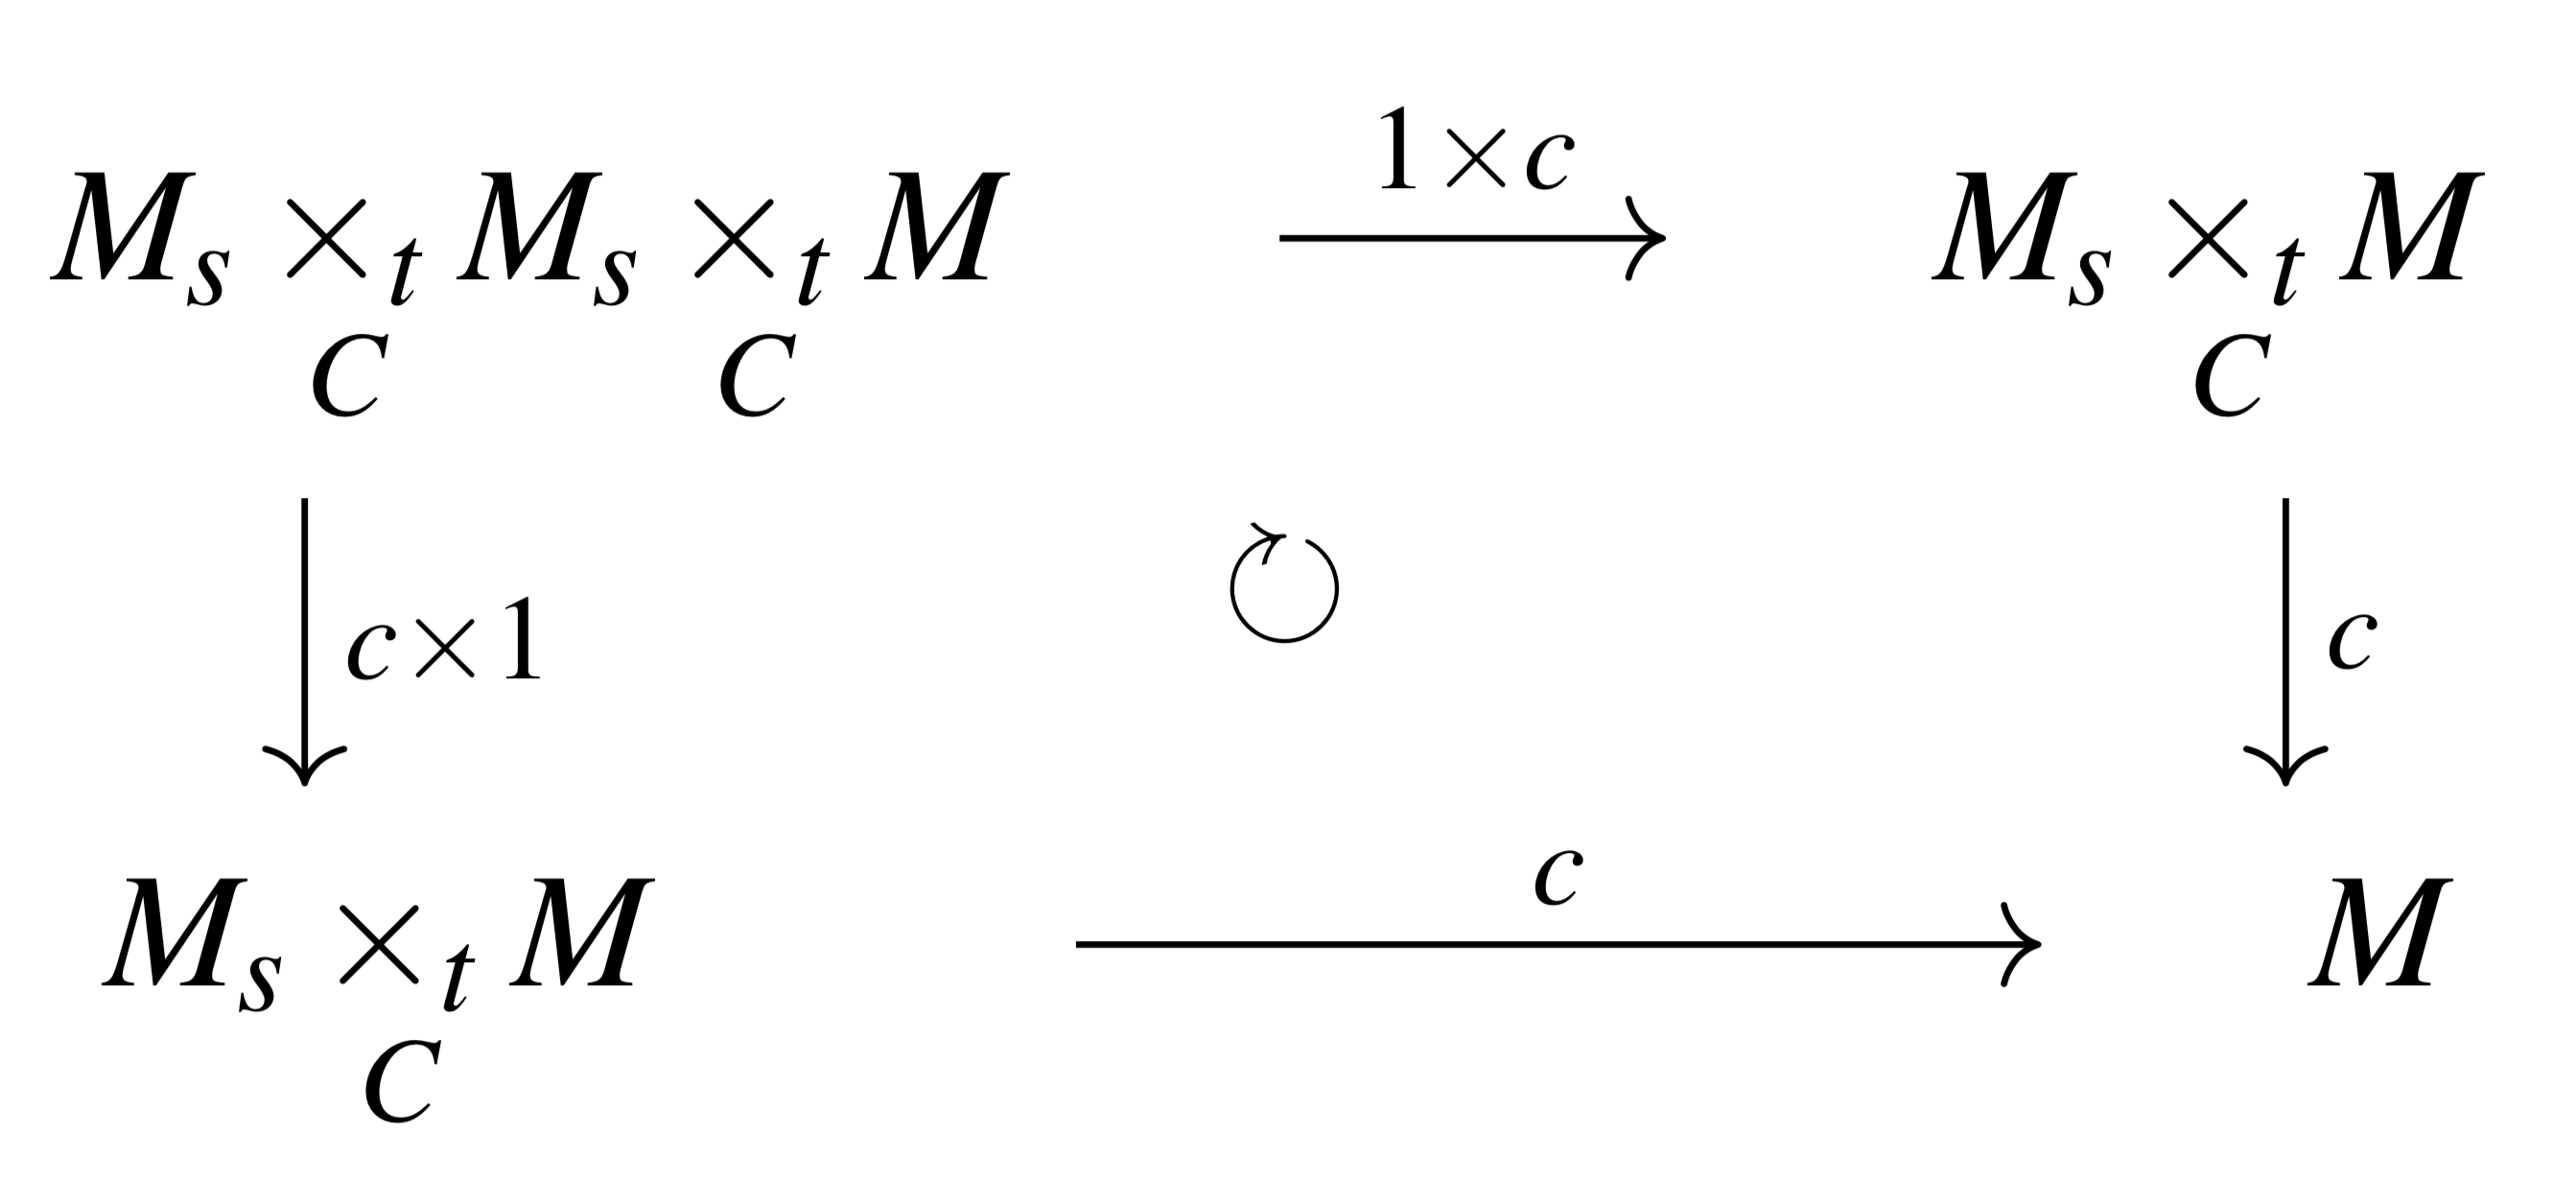
\includegraphics[width=7cm]{cd-2.png}
\end{center}\end{figure}
但し,$M_s \underset{C}{\times_t}M_s \underset{C}{\times_t}M := \{ (h,g,f)\in M\times M\times M : \; s(h)\overset{c}{=} t(g) \wedge \; s(g) \overset{c}{=} t(f) \}$であり,$$\begin{array}{ccc}
        c\times1:M_s\underset{C}{\times_t}M_s\underset{C}{\times_t}M & \longrightarrow & M_s\underset{C}{\times_t}M \\
        \rotatebox{90}{$\in$} & & \rotatebox{90}{$\in$}\\
        (h,g,f) & \longmapsto & (c(h,g),f) \\[3mm]
        1\times \! c:M_s\underset{C}{\times_t}M_s\underset{C}{\times_t}M & \longrightarrow & M_s\underset{C}{\times_t}M \\
        \rotatebox{90}{$\in$} & & \rotatebox{90}{$\in$}\\
        (h,g,f) & \longmapsto & (h,c(g,f))
\end{array}$$

これがwell-definedである理由は,図\ref{def-cd:1}より,$s(g)=s(c(h,g))=t(f)$が保証されているから,$(h,g,f)$は確かに必ず$M_s \underset{C}{\times_t}M_s \underset{C}{\times_t}M$に含まれるのである.\\[3cm]

\begin{figure}[ht] \begin{center}  \caption{\label{def-cd:3} 単位射$e$の存在.4つの写像について,$s\circ e=1_c=t\circ e$の関係を表す可換図式.}
    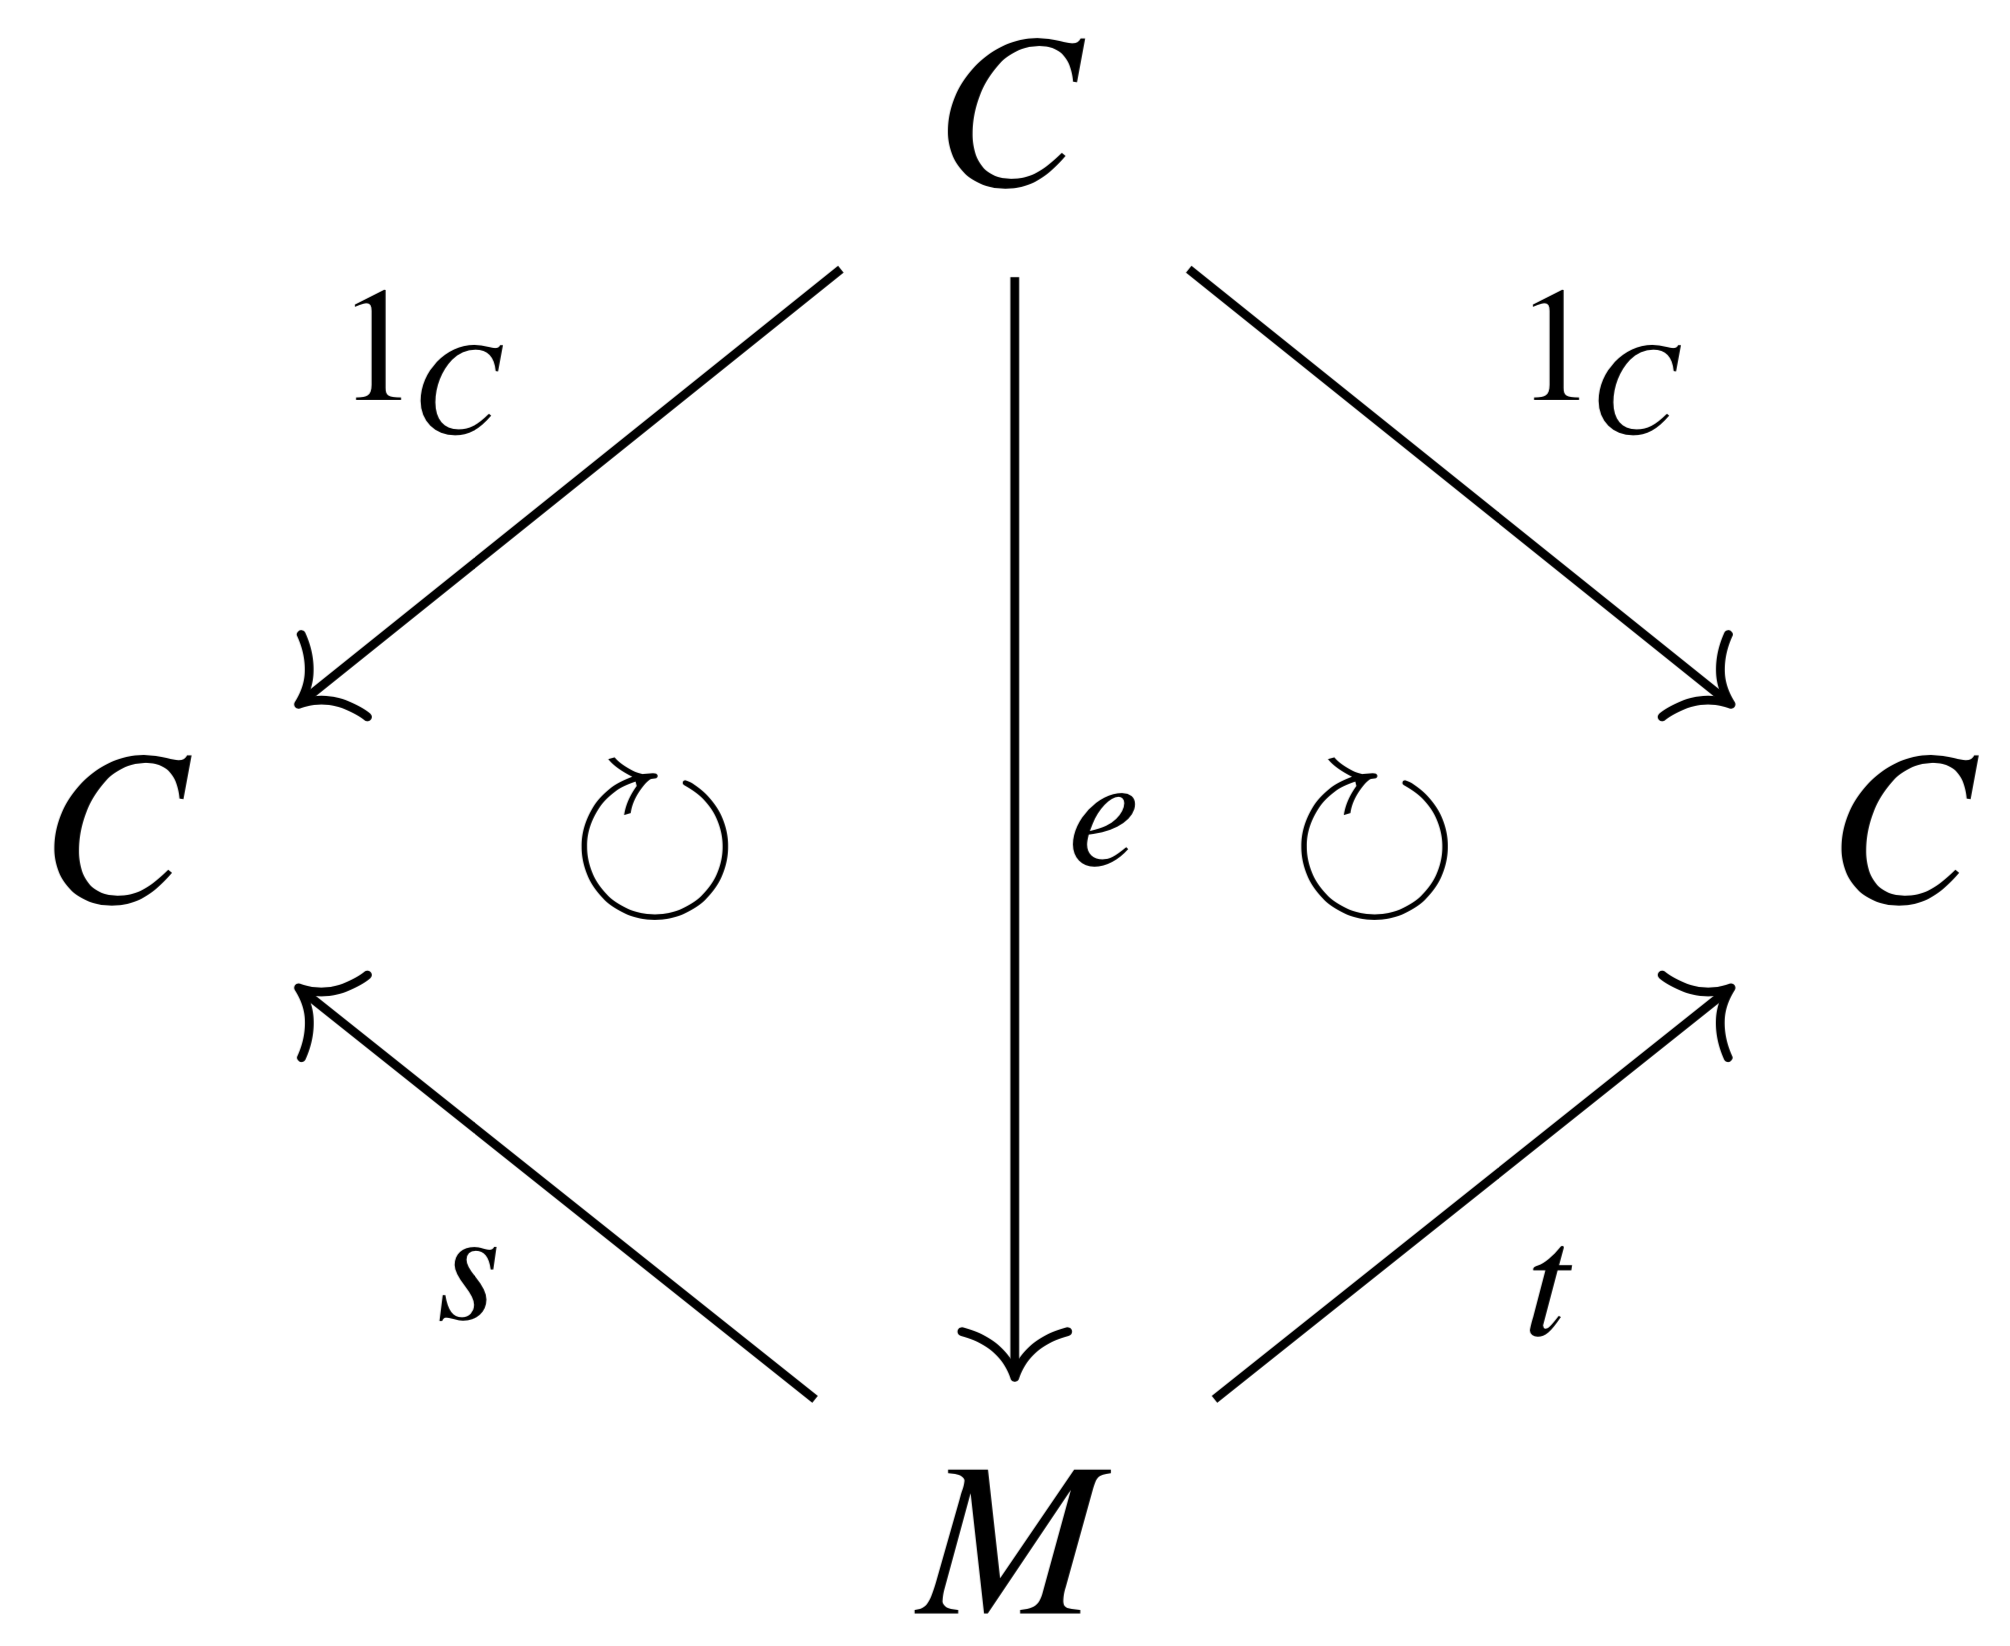
\includegraphics[width=7cm]{cd-3.png}
\end{center}\end{figure}
つまり,$C$の任意の元を$A$と取ると,$A=1_c(A)=s(e(A))=t(e(A))$だから,つまり,射$e(A)$は$e(A):A\longrightarrow A$である.このような射のうち特別なものを1つ定めて恒等射と呼び,図\ref{def-cd:3}によると全ての$C$の元について定まる.この特別な自己射の特徴付け(正確に同じものは同じものに写す自己愛写像であること)は次で定める.

\begin{figure}[ht] \begin{center}  \caption{\label{def-cd:4} 単位射$e$の特徴付け.$c(e(t(f)),f)=c(f,e(s(f)))$,即ち勝手な$M$の元を$f:A\longrightarrow B$と置いた時に,$f\circ e(A)=e(B)\circ f$(恒等射$e(A)$の特徴付け/interface)を表す可換図式.}
    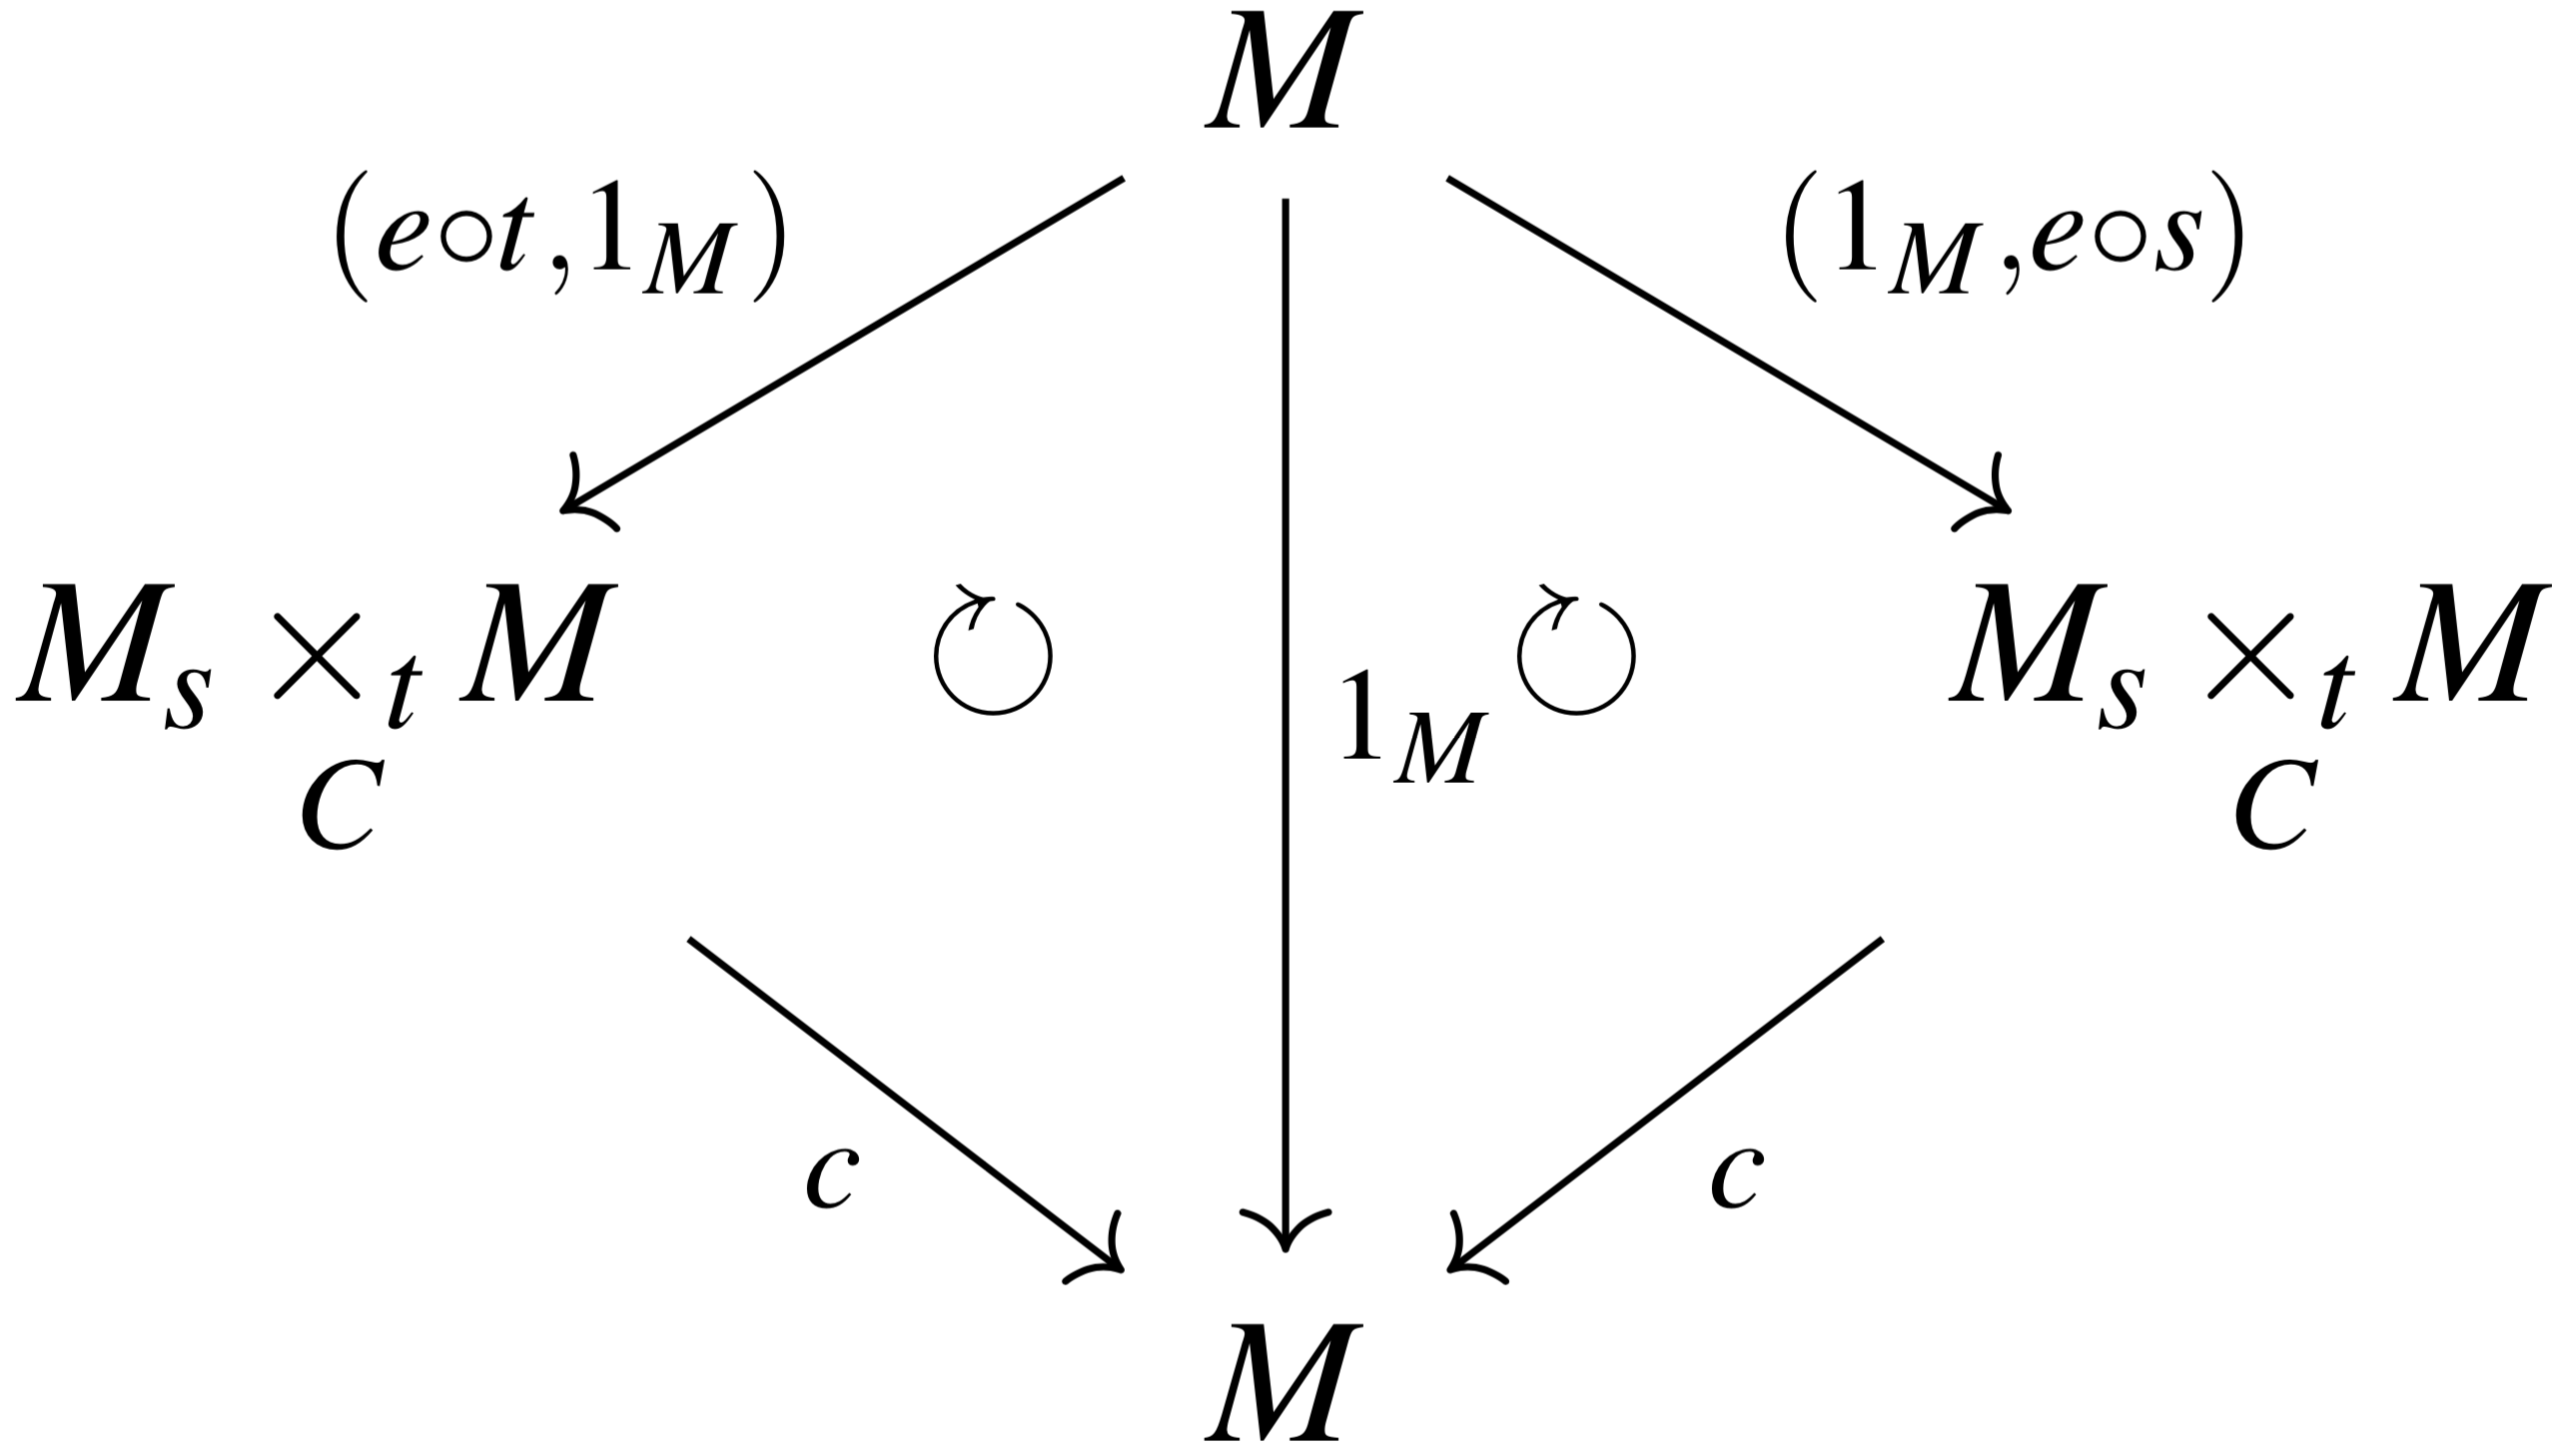
\includegraphics[width=7cm]{cd-4.png}
\end{center}\end{figure}
但し,$e\circ s:M\xrightarrow{\quad s\quad}C\xrightarrow{\quad e \quad}M$であり,
$\begin{array}{ccc}
    (1,e\circ s):M & \longrightarrow & M_s \underset{C}{\times_t}M\\
    \rotatebox{90}{$\in$} & & \rotatebox{90}{$\in$}\\
    f & \longmapsto & (f,e(s(f)))
\end{array}$
である.

\subsection{ここで一息,定義の吟味.記法の集合論との混用.}

結局,集合論的に言い直せば,$C=ob(\mathcal{C})$,$M=arr(\mathcal{M})$,$s,t$(\underline{s}ource, \underline{t}arget)は全ての射に,夫々「始対象」と「終対象」という対象を紐付ける写像$s,t:M\longrightarrow C$,$c$は始対象と終対象が一致する射の組について必ず或る別の射(合成)を対応させる写像$c:M_s \underset{C}{\times_t}M \longrightarrow M$,$e$は対象の一つ一つについて或る射(恒等射)を対応させる写像$e:C\longrightarrow M$(たった一つを選び取る)である.\\
射に付随する2つの対象「始対象」「終対象」を$s,t$,各対象に結び付けられた特別な射「恒等射」を$e$と言う選択関数/特性関数,合成と言う演算を$c$と言う写像と見なして,その性質を可換図式で語る,と言う枠組みで圏の定義をした.

$f\in M$の時,$s(f), t(f)\in C$であるが,この関係を$f:s(f)\longrightarrow t(f)$と書いて(写像の記法と混用.写像も射と見做せるが,射の方が高次元の用語である.),「$f$は$s(f)$から$t(f)$への射である」という.$C$の元である$s(f),t(f)$を以降,夫々アルファベットの大文字で$A,B$などと書くこととする.\\
$c(g,f)$は以降,写像の合成と混用して,$g\circ f$と書く.$A\in C$に対して,恒等写像の記号を混用して,$e(A)=:1_A : A\longrightarrow A$と書く.\\
また,圏$C$と言った時は,$C$を対象の集合とみなしている場合が多い.

\clearpage
\section{圏の例}
おしなべて,数学理論は何か世界の「型(type)」について議論をする.様々な具体的対象が,その型に当てはまれば,例に漏れず必ず普遍的にもつ性質について考えたいからだ.\\
例を見ていくと分かる通り,圏論は特に抽象的だしスケールがでかい.これらの例を確認してから,「じゃあこいつらの型に,共通して言えるものはなんだろう?」と考えたい.

\subsection{集合の圏\bf{Sets}}

$C$:小さな集合全体の集合 とする.(すると$C\in\mathfrak{U}$)\\
$A,B,D\in C$に対して,$\mathrm{Mor}_c(A,B)=\mathrm{Map}(A,B)$とし,$$\begin{array}{lcr}\circ : \mathrm{Map}(B,D)\times\mathrm{Map}(A,B)&\longrightarrow&\mathrm{Map}(A,D)\\ \hspace{16mm}\rotatebox{90}{$\in$} & & \rotatebox{90}{$\in$}\\ \hspace{13mm}(g,f) & \longmapsto & g\circ f \end{array}$$
と言うように射の合成を自然に定義し,恒等射は恒等写像$1_A:A\longrightarrow A$とすると,これは圏をなす.

\subsection{線型代数学からの例}

$C$:有限次元実線型空間全体の集合 とする.\\
$V,W\in C$について,$\mathrm{Mor}_c(V,W)=\mathrm{Hom}_\mathbb{R}(V,W)$とし,他射の合成と恒等写像$1_V$については前述の集合の圏と同様にすれば,これは圏をなす.

\subsection{微積分学からの例}

$C$:$\mathbb{R}^2$上の開集合$U$全体の集合 とする.\\
$U,V\in C$に対して,射の集合を$\mathrm{Mor}_c(U,V)=\{f:U\longrightarrow V: f\text{は連続微分可能な写像}\}$と定める.\\
すると,集合としての写像の合成と,恒等写像を$1_U:(x,y)\longmapsto (x,y)$とすれば,これは圏をなす.

\subsection{用語の補充:同型射}

\begin{shadebox}\begin{definition}[可逆,同型,逆射]
    射$f:A\longrightarrow B$に対して,射$g:B\longrightarrow A$であって,$g\circ f=1_A \; \wedge \; f\circ g=1_B$となる射$g$が存在するとき,$g$を「逆射」といい,$f$は可逆である/同型射である,と言う.
\end{definition}\end{shadebox}

今までの例は,「(集合論,線型代数学,微分積分学など)数学の大きな理論の中から,圏の構造を見出す」と言う構図であったが,以降の例は,圏そのものと見做せる代数的構造の例を挙げる.

\subsection{monoidという圏}

$C={A}$と言う一点集合とする.\\
したがって,$s,t$は定値写像(値(value)が常にAである写像)となる.つまり,特に$s(g)=t(f)=A$が成り立つ.\\
これにより,$c$の定義域は$M_s\underset{C}{\times_t}M=\{ (g,f)\in M\times M : s(g)=t(f)=A \}=M\times M$より,$c:M\times M\longrightarrow M$であり,$e:C\longrightarrow M$は射の中から特別な1つを適当に選び出すだけである.これを$e:=e(A)=1_A$と書くこととする.\\
以上より,結局,後は$(h\circ g)\circ f = h\circ (g\circ f)$と$f\circ e=e\circ f = f$を充たす3-組$<M,\circ :M\times M\longrightarrow M,e>$の取り方1つ1つに対して,圏$C$が1つずつ定まる.\\
これはモノイド全体と一致する.\\

\begin{screen}
    対象の集合$C$が一点集合である場合の圏全体は,モノイド$M$全体のことである.\\
    なお,モノイド$M$の全ての元が可逆であった時,$<M,\circ,e>$を特に群と言う.
\end{screen}

これは,普段は集合論的に構成される代数的対象たちの,圏論からのまとめ直しである.\\
この立場からは,群の公理の3つ目は,逆元の存在というよりも,逆射の存在として捉えられる.\\
ただ,この公理を体の公理の1つとして見る時,あるいはモノイドの例として$<\mathbb{N},+>$,群の例として$<\mathbb{Z},+,0>$を考えるとき,我々は数の一つ一つを射だとは,あまり見なさない出来た.やはりobjectとしての実感を持ったものというイメージは初源的なのだろうか.

\subsection{順序関係}

$C$:集合 とし,$M\subset C\times C$とする.第一射影と第二射影,つまり$\begin{array}{llccrr} s:M & \longrightarrow & C & t:M & \longrightarrow & C \\ \rotatebox{90}{$\in$} & & \rotatebox{90}{$\in$} & \rotatebox{90}{$\in$}& & \rotatebox{90}{$\in$}\\ (x,y) & \longmapsto & x & (x,y) & \longmapsto & y \end{array}$によって$s,t$を定める.\\
この下で,$<C,M,s,t,c,e>$が圏をなし,\underline{さらに全ての同型射は単位射である(=逆射を持つならそれは単位射である)時},「$M$は$C$の順序を定める」という.\\

つまり,$x,y\in C$に対して,$(x,y)\in M$の時,$x\le y$と書くこととする.(二項関係も射である)\\
$x\le y \wedge y\le z \Longrightarrow x\le z$という二項関係の推移性は,射の合成に当たる.\\
ここまでで「前順序(pre-order)」と呼ぶが,そして下線部の条件により,$x\le x \wedge x\ge x \Longrightarrow x=x$つまり,$M\ni 1_x:x\longmapsto x$が満たされる.

大抵の構造は射の言葉で語れる,非常に良い例だ.

\clearpage
\section{関手(functor):圏準同型}

\begin{shadebox}\begin{definition}[関手]
    2つの圏$C=(C,M,s,t,c,e),C'=(C',M',s',t',c',e')$に対して,圏$C$から圏$C'$への関手とは,写像$F_C:C\longrightarrow C'$と写像$F_M:M\longrightarrow M'$の組$(F_C,F_M)=:F$であって,以下の可換図式\ref{cd-5},\ref{cd-6},\ref{cd-7}を満たすもののことである.
\end{definition}\end{shadebox}

\begin{figure}[ht]\begin{center} \caption{\label{cd-5} 射に付随する始対象と終対象との関係を保存すること.}
    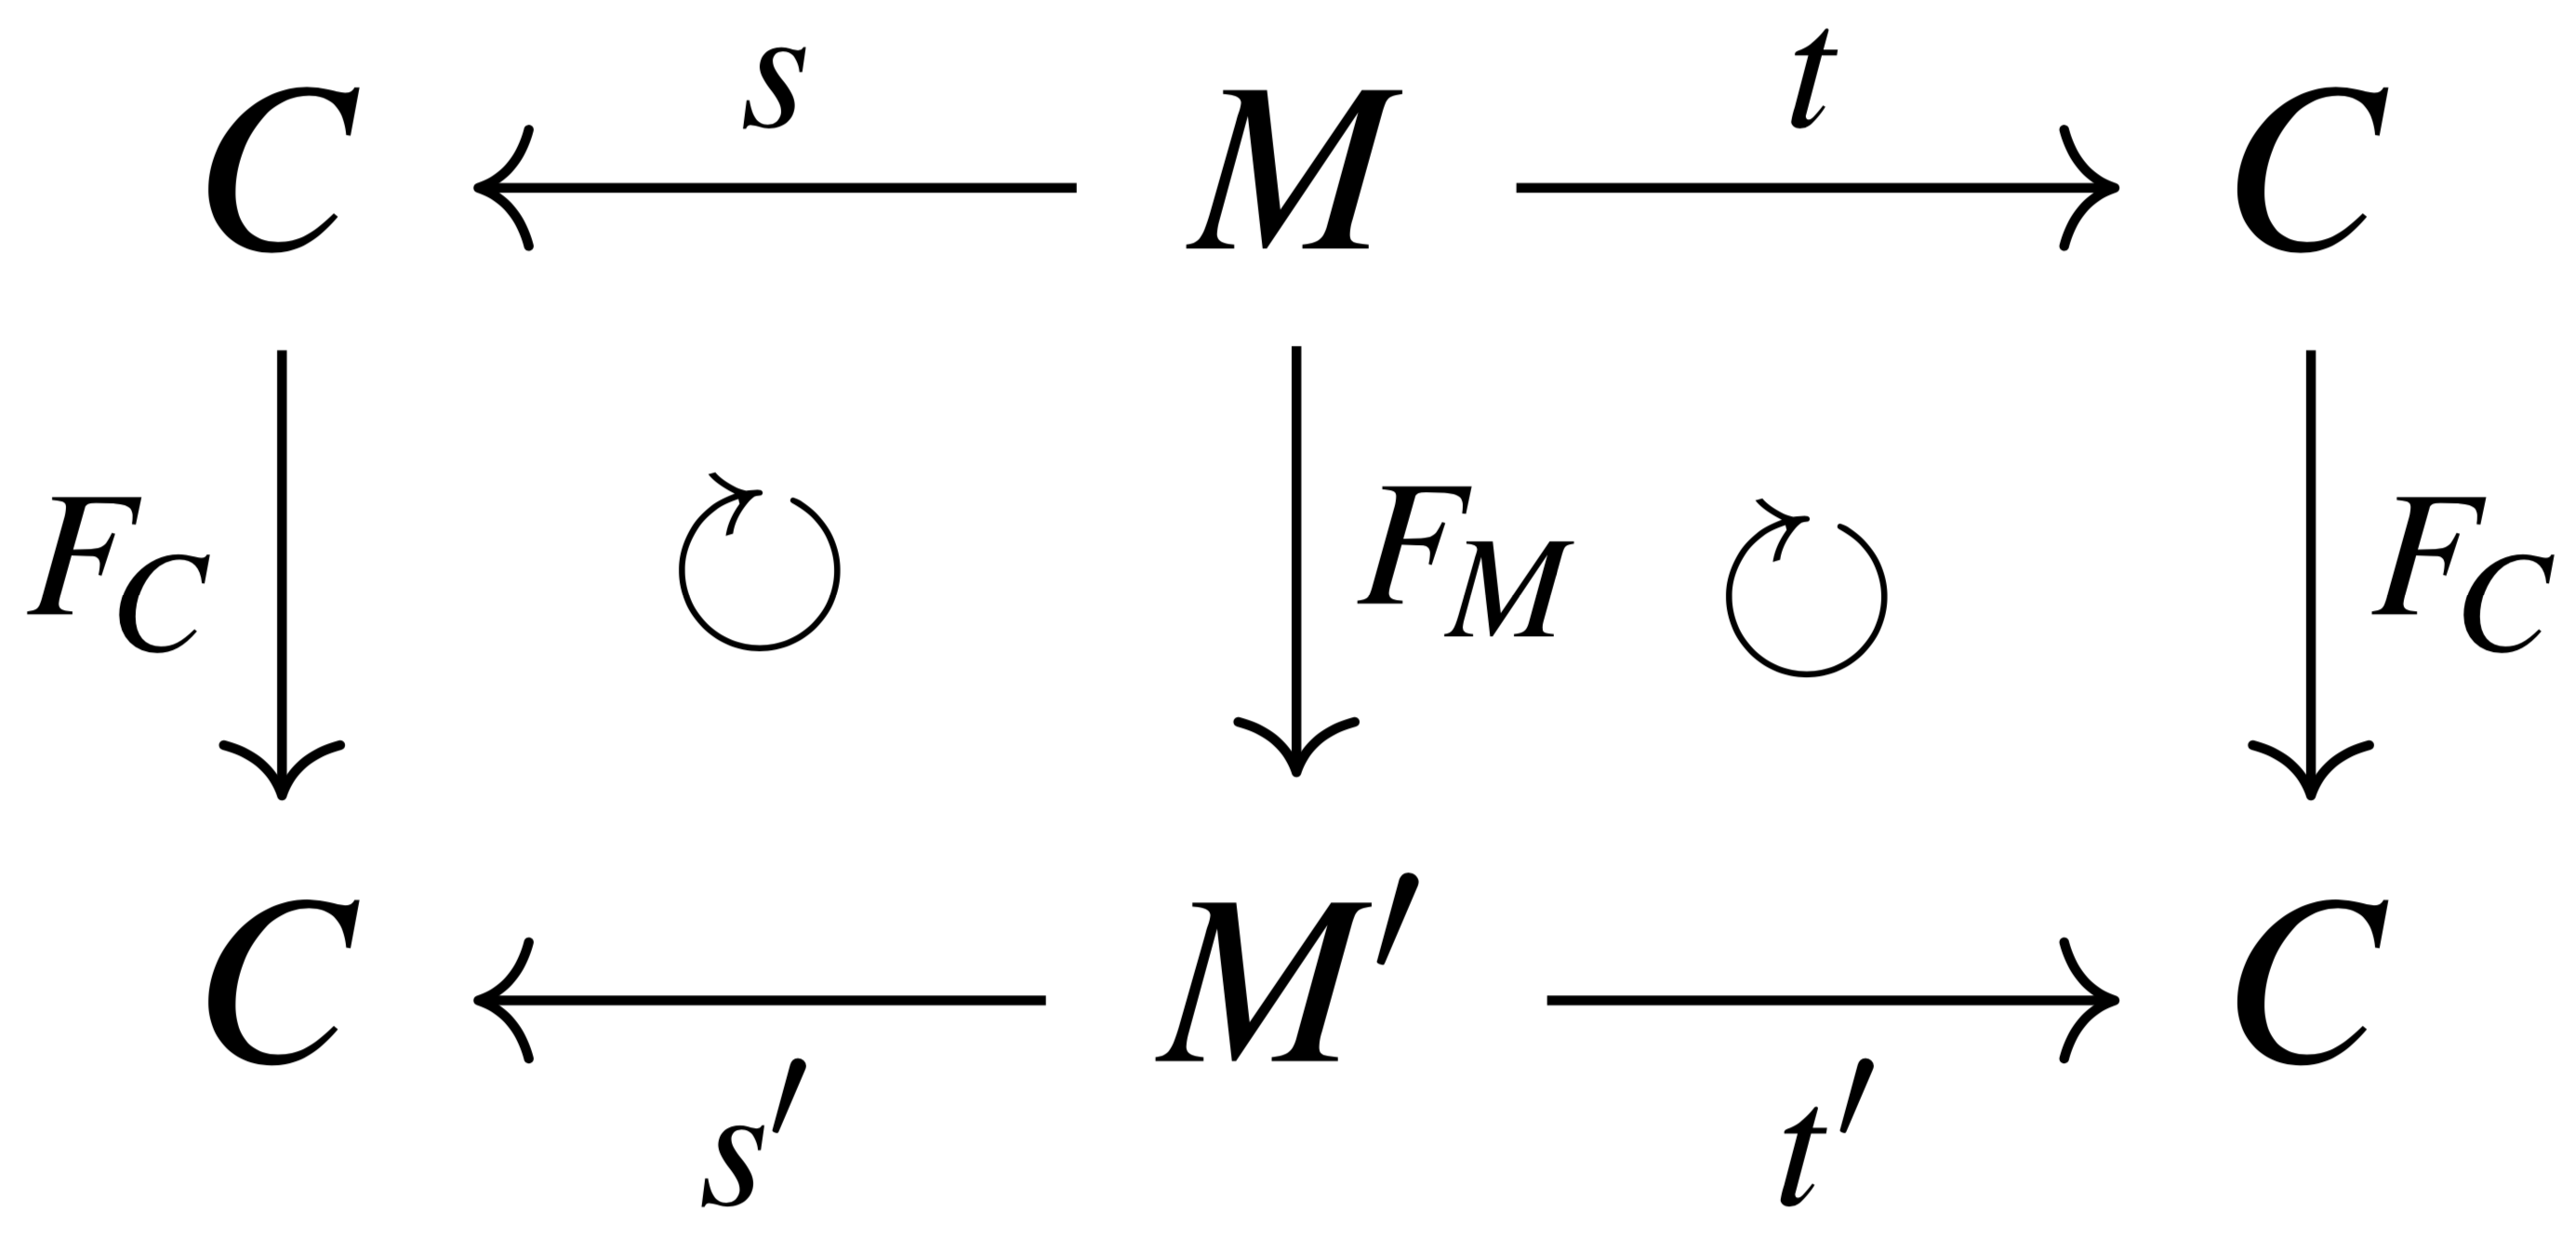
\includegraphics[width=7cm]{cd-5.png}
\end{center}\end{figure}

\begin{figure}[ht]\begin{center} \caption{\label{cd-6} 射の合成が可換である.先に合成しても,後で合成しても同じことである.}
    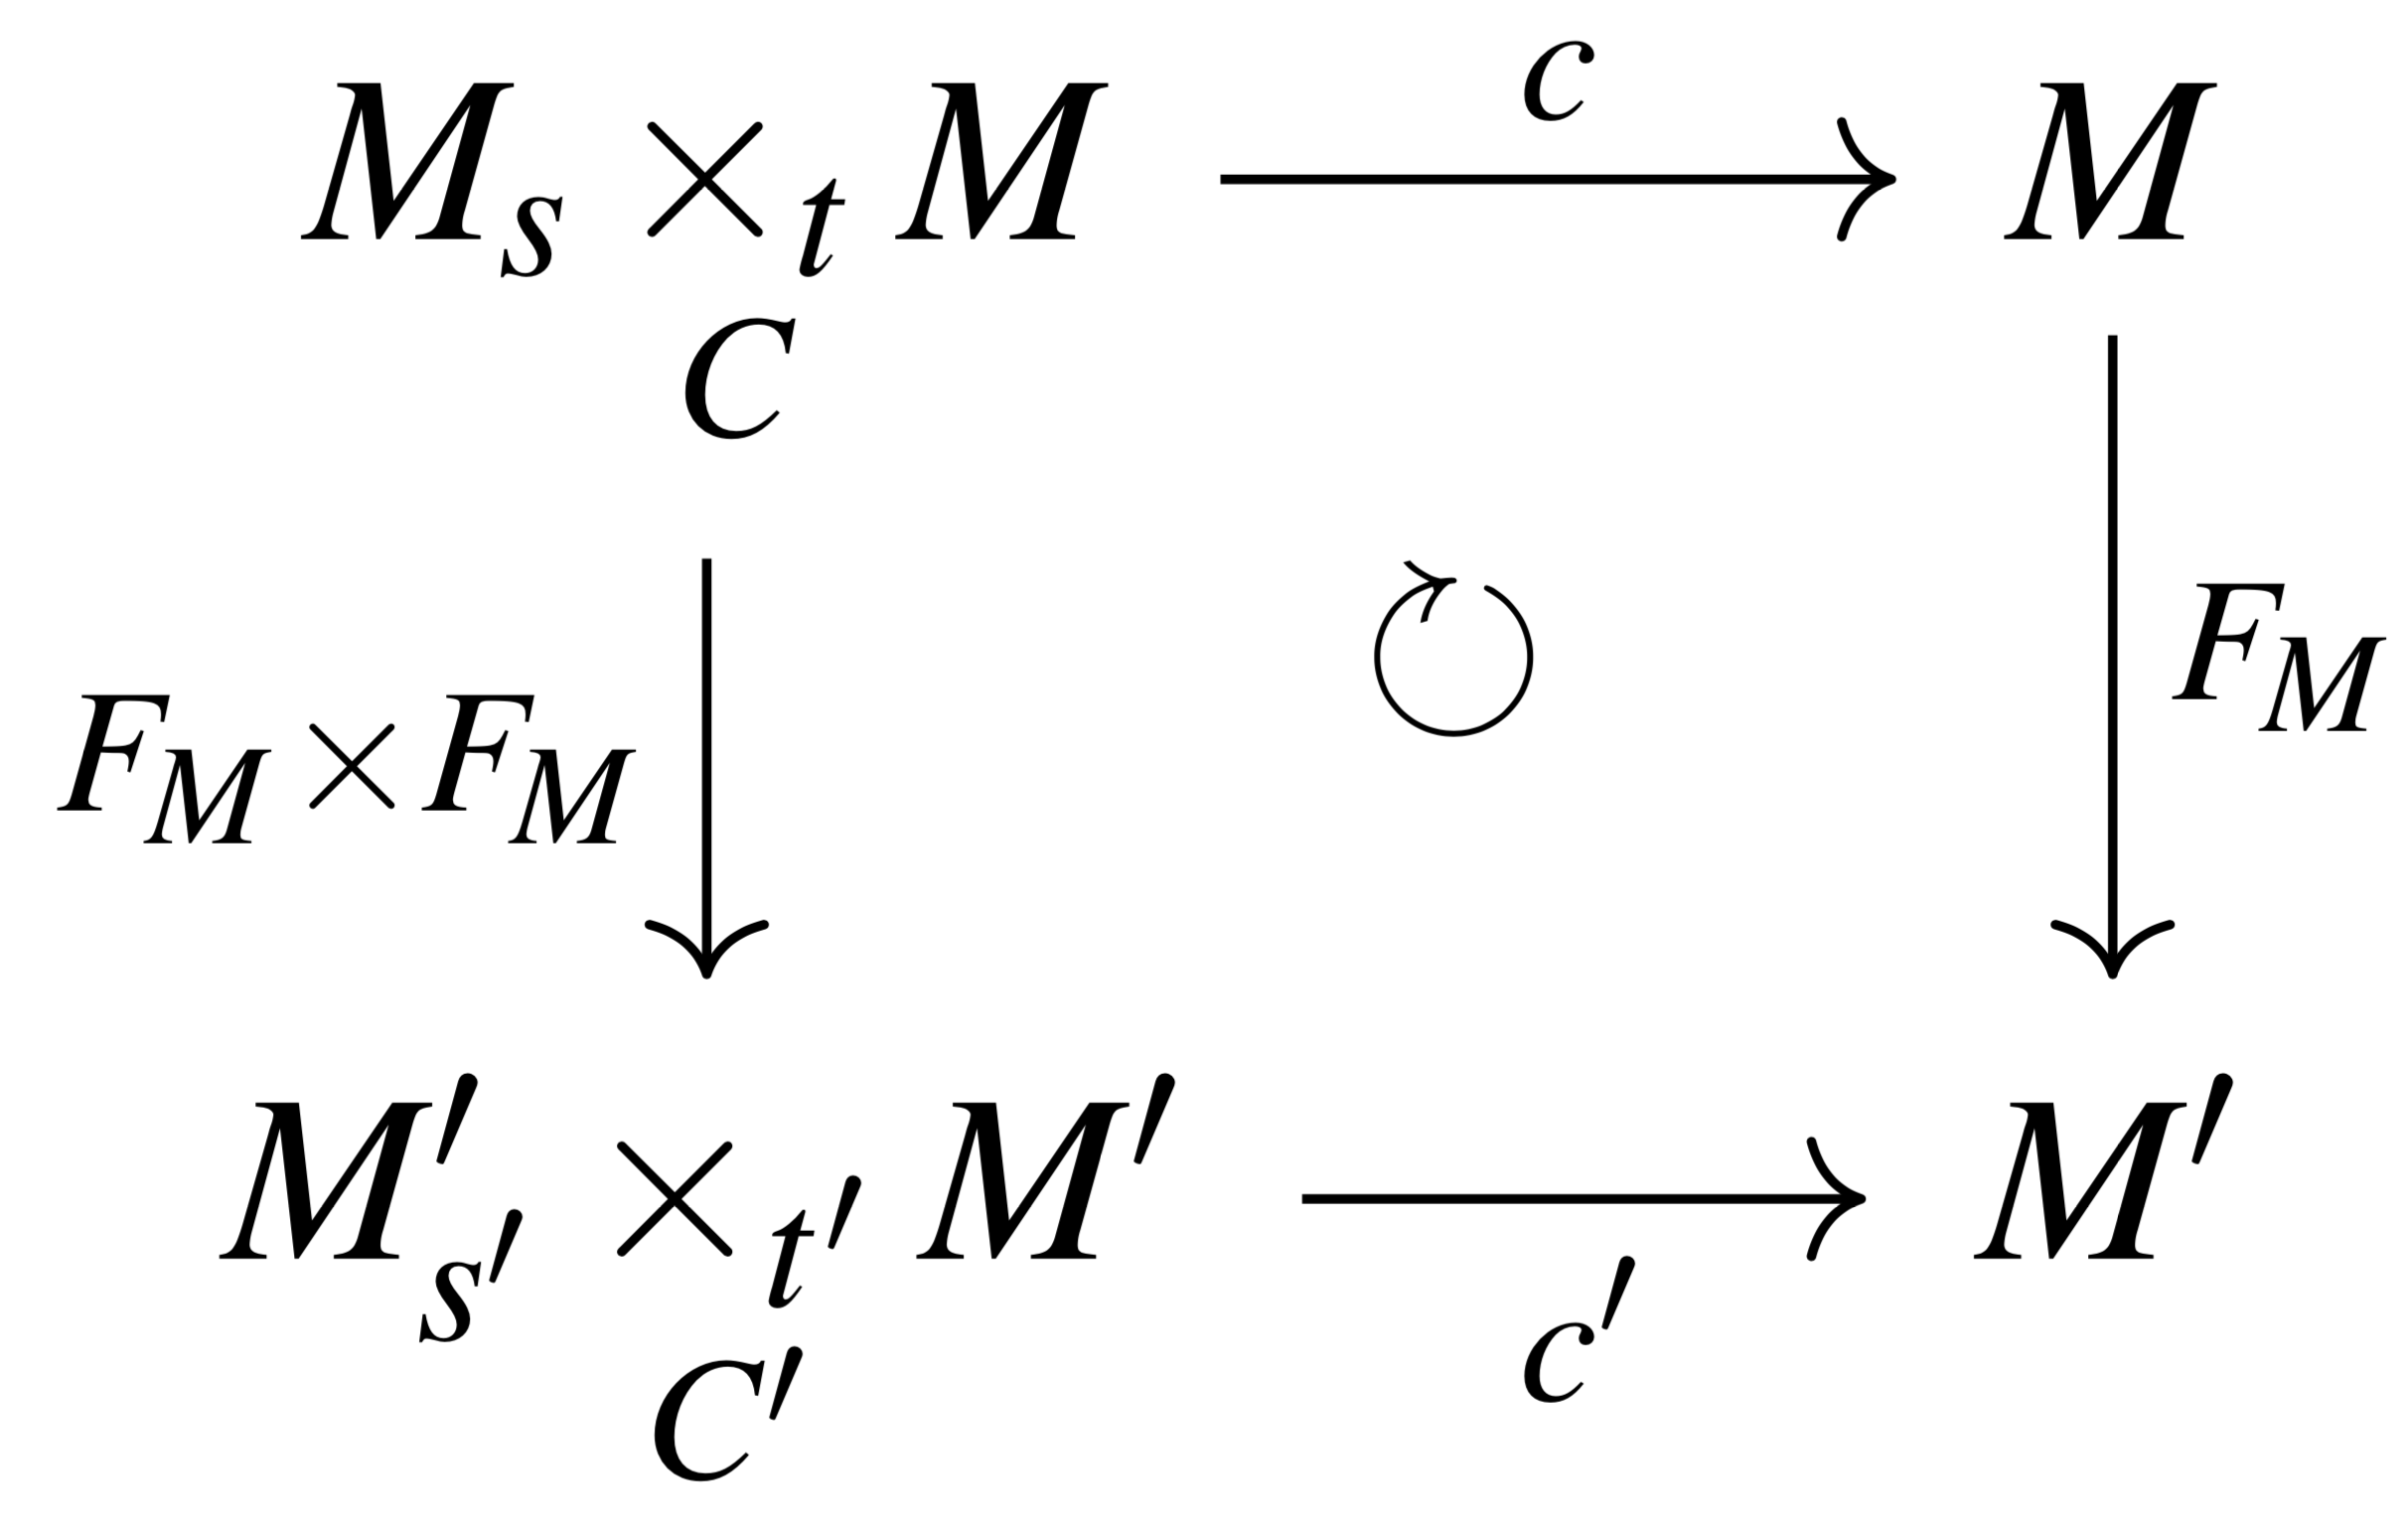
\includegraphics[width=7cm]{cd-6.png}
\end{center}\end{figure}

\begin{figure}[ht]\begin{center} \caption{\label{cd-7} 単位射は単位射に対応する.}
    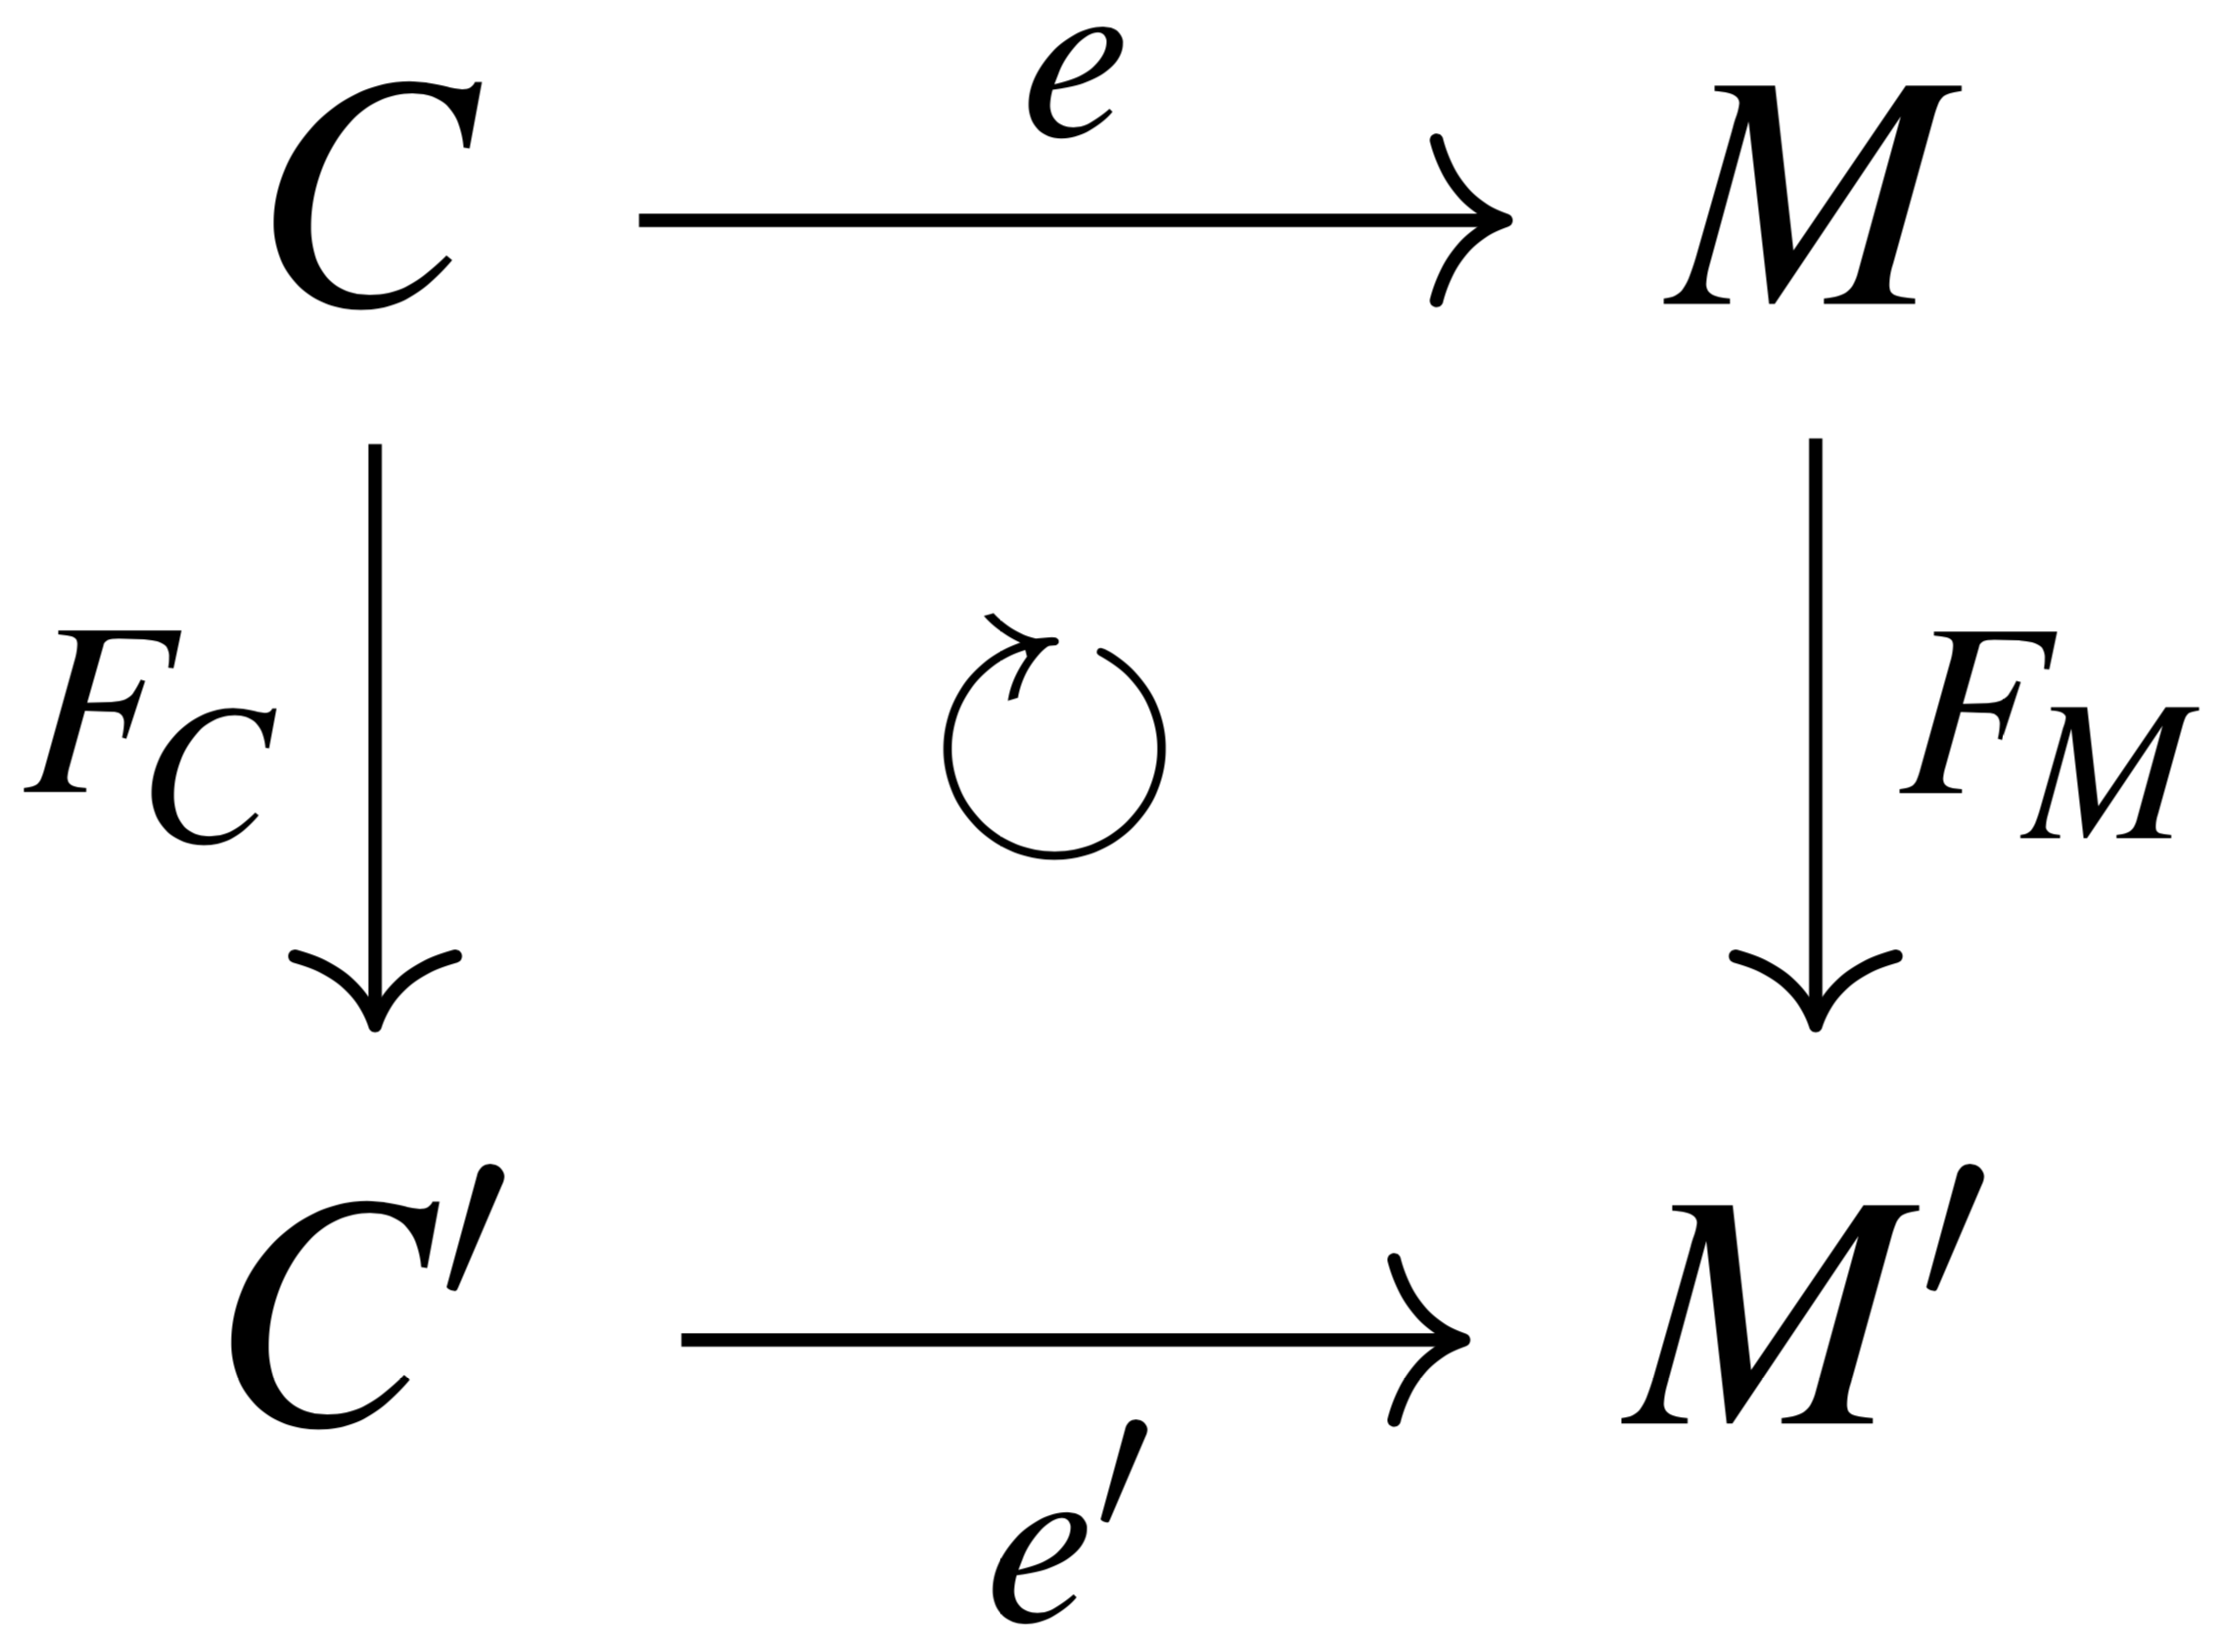
\includegraphics[width=5cm]{cd-7.png}
\end{center}\end{figure}

以上,3つの構造を保つ写像(の組)が関手であるから,まさに圏の間の準同型である.

\end{document}